
\documentclass[12pt]{article}
\setlength\parindent{0pt}
\usepackage{fullpage}
\usepackage{amsmath}
\usepackage[margin=0.5in, paperwidth=13.5in, paperheight=8.4in]{geometry}
\usepackage{graphicx}
\setlength{\parskip}{4mm}
\def\LL{\left\langle}   % left angle bracket
\def\RR{\right\rangle}  % right angle bracket
\def\LP{\left(}         % left parenthesis
\def\RP{\right)}        % right parenthesis
\def\LB{\left\{}        % left curly bracket
\def\RB{\right\}}       % right curly bracket
\def\PAR#1#2{ {{\partial #1}\over{\partial #2}} }
\def\PARTWO#1#2{ {{\partial^2 #1}\over{\partial #2}^2} }
\def\PARTWOMIX#1#2#3{ {{\partial^2 #1}\over{\partial #2 \partial #3}} }
\newcommand{\BE}{\begin{displaymath}}
\newcommand{\EE}{\end{displaymath}}
\newcommand{\BNE}{\begin{equation}}
\newcommand{\ENE}{\end{equation}}
\newcommand{\BEA}{\begin{eqnarray}}
\newcommand{\EEA}{\nonumber\end{eqnarray}}
\newcommand{\EL}{\nonumber\\}
\newcommand{\la}[1]{\label{#1}}
\newcommand{\ie}{{\em i.e.\ }}
\newcommand{\eg}{{\em e.\,g.\ }}
\newcommand{\cf}{cf.\ }
\newcommand{\etc}{etc.\ }
\newcommand{\Tr}{{\rm tr}}
\newcommand{\etal}{{\it et al.}}
\newcommand{\OL}[1]{\overline{#1}\ } % overline
\newcommand{\OLL}[1]{\overline{\overline{#1}}\ } % double overline
\newcommand{\OON}{\frac{1}{N}} % "one over N"
\newcommand{\OOX}[1]{\frac{1}{#1}} % "one over X"

\pagenumbering{gobble}

\begin{document}
\Large
\centerline{\sc{Recitation Exercises}}
\normalsize
\centerline{\sc{Friday, 30 April}}

Earlier in our class, we have concerned ourselves with applying kinematics to situations when {\it acceleration is constant}. This is because the calculus is very easy:

\begin{align*}
\text {acceleration} &= \text{constant} &   a(t )&= a \\
\text {velocity} &= \text{integral of acceleration} & v(t) = \int\,a\, dt  &= at + v_0 \\
\text {position} &= \text{integral of velocity} & x(t) = \int\,(at + v_0)\,dt &= \frac{1}{2}at^2 + v_0 t + x_0
\end{align*}

This allows us to calculate everything about the motion of objects where the forces do not change over time.

In an early homework set, you saw that if the acceleration changes with time in a known way-- say, $a(t) = \beta t$ -- you could take two integrals of that function and find other kinematics equations. 


\newpage

For instance, in a situation where the acceleration $a(t) = \beta t$:


\begin{align*}
\text {acceleration} & &    a(t )&= \beta t \\
\text {velocity} &= \text{integral of acceleration} & v(t) = \int\,a\, dt  &= \frac{1}{2}\beta t^2 + v_0 \\
\text {position} &= \text{integral of velocity} & x(t) = \int\,\left(\frac{1}{2}\beta t^2 + v_0\right)\,dt &= \frac{1}{6} \beta t^3 + v_0 t + x_0
\end{align*}
\bigskip

Let's consider now a situation where an object of mass $m$ is connected to a spring of spring constant $k$ on a frictionless table. We know that if you pull the mass to the side, it will bounce back and forth; in today's exercise, we will see how this oscillatory motion results from the laws of physics you already know.

For simplicity, let's use a coordinate system where $x=0$ corresponds to the equilibrium position of the spring. Our goal will be to calculate an expression for {\it position as a function of time} -- that is, $x(t)$ for this system.


{\bf 1.}
\begin{minipage}{0.4\textwidth}
Write down an expression for the force on the mass in this coordinate system. (This will be very simple!) Remember that the force is in the {\it opposite direction} of the displacement.
\end{minipage}
\hspace{0.1\textwidth}
{\bf 2.}
\begin{minipage}{0.46\textwidth}
Now, using Newton's law, solve for the {\it acceleration} of the system. Once you have a result, call your TA or coach over and ask them to check your result. 
\end{minipage}

\vspace{1in}



Above, we saw that if you know the {\it acceleration as a function of time}, you can take two integrals to find the position as a function of time (the thing we want). Explain why the above approach will not work here. 

\vspace{1in}
\newpage
Since we can't use the thing we already know, we will have to figure something else out! Our problem is that the acceleration is now a function of {\it position}. We know what to do if we know $a(t)$ -- but now we know $a(x)$:

We don't quite know what to do with this! The biggest problem is that $x$ -- an unknown function of time -- appears on the right-hand side, so {\it both} sides of this equation have things we do not know.

$$a(x) = -\frac{k}{m}\,x(t)$$

The easiest approach is to replace acceleration with its definition as ``the second derivative of position with respect to time'', and then ask ``what kind of function can I put in here that will work?'' There are two ways that you might do this:

\vspace{0.3in}

\begin{center}\underline{\hspace{6in}}\end{center}

\begin{minipage}{0.46\textwidth}

In math class, you probably learned to write time derivatives this way:

\begin{align*}
\frac{dx}{dt} &\equiv v \\
\frac{d^2x}{dt^2} &\equiv a 
\end{align*}
\end{minipage}
\begin{minipage}{0.46\textwidth}
In physics we sometimes use a simpler notation using dots above the variable to represent time derivatives:

\begin{align*}
\dot x &\equiv v \\
\ddot x &\equiv a 
\end{align*}

Physicists and engineers usually do {\it not} write $\frac{dx}{dt}$ as $x'$.



\end{minipage}
\begin{center}\underline{\hspace{6in}}\end{center}

\vspace{0.3in}

Using either notation from above, replace acceleration by its definition as the second derivative of position. 

\newpage

On the previous page, you found that

\begin{align*}
\frac{d^2 x}{dt^2} &= -\frac{k}{m}\,x(t) &or&& \ddot x(t) &= -\frac{k}{m}\,x(t) 
\end{align*}

These equations relate a function to its second derivative. We need to find some function $x(t)$ that satisfies the following:

\large \bf ``When I take the second derivative of $x(t)$, I get that same function back, but with a negative sign, and multiplied by $\frac{k}{m}$'' \rm \normalsize

It turns out that in situations like this, the easiest way to figure it out is to just {\it guess the answer!} The way to do this is a two-step process:

\begin{enumerate}
	\item Consider ``template'' functions that have unknown parameters in them -- for instance, a generic exponential might be $x(t) = Ae^{\beta t}$, with $A$ and $\beta$ unknown -- and find one with the right properties.
	\item Plug your template into the equation $\ddot x(t) = -\frac{k}{m}\, x(t)$ and figure out what the unknown parameters are
\end{enumerate}

\vspace{0.5in}

\newpage

Here are some template functions that you might consider. Your goal is to find a function that satisfies:


\large \bf ``When I take the second derivative of $x(t)$, I get that same function back, but with a negative sign, and multiplied by $\frac{k}{m}$'' \rm \normalsize


	\large
	\begin{center}
\begin{tabular}{llll}

\hspace{2in} & \hspace{2in} & \hspace{2in} \\ 

\vspace{1em}

$x(t) = A \tan (\omega t)$ & $x(t) = Ae^{\beta t}$ & $x(t) = Ae^{-\beta t}$ & $x(t) = A \sqrt {\beta t + \gamma t^2}$  \\
\vspace{1em}
$x(t) = A \cos (\omega t)$ & $x(t) = A + Bt + Ct^2$ & $x(t) = A + Bt + Ct^2 + Dt^3$ & $x(t) = A\sqrt{\beta t}$\\
\vspace{1em}
$x(t) = A \sin (\omega t)$ & $x(t) = A \ln \frac{t}{\tau}$ & $x(t) = \frac{\tau}{t}$ & $x(t) = A\frac{t+B}{t-C}$ \\

\end{tabular}

\end{center}

\normalsize

Remember, your goal is to find a function that, when you take two derivatives, gives back {\it that same function}, with a minus sign, and multiplied by something. Consider each of the templates; cross ones out that don't work, and circle the ones that do have the properties you are looking for. As a hint, think about the behavior of each of these functions (what does the graph look like?), and think about how you expect a mass connected to a spring to behave.

Which function(s) work? Are they the ones you expect?

\vspace{1in}

Now, we need to find out what the unknown variables (A, B, C, D, $\beta$, $\tau$, $\omega$) might be in your template function(s). Take two derivatives of your function(s). For instance, the second derivative of $Ae^{\beta t}$ is $A\beta^2e^{\beta t}$. 

\vspace{1in}

\newpage

Substitute your function back into the equation you started with: $\ddot x(t) = -\frac{k}{m}\,x(t).$ Then solve for your unknowns (for instance, what is $\omega$?)


\vspace{1in}

You will find that $A$ could have any value at all. This is fine! It means that a function with any value of $A$ satisfies the equation we started with.

Remember that we are figuring out what happens when a mass bounces back and forth on a spring. Does it make physical sense that $A$ could be either large or small?

\vspace{1in}

Our choice to use the variable $\omega$ here was not an accident. This is called the {\it angular frequency} of the oscillations; large values of $\omega$ result in faster oscillations and smaller values result in slower ones. Look at your formula for $\omega$ as a function of $k$ and $m$. Does it change the way you expect when $k$ increases (the spring gets stiffer)? Does it change the way you expect when $m$ increases (the mass gets more massive)?

\vspace{0.8in}

\begin{minipage}{0.6\textwidth}
Here is an example graph of $x(t)$ with $\omega=1\, \frac{\text{rad}}{\text {s}}$ and $A = 1$ cm. On this graph, label:

\begin{itemize}
\item A point where the kinetic energy is zero and all the energy is elastic potential energy
\item A point where the potential energy is zero and all the energy is kinetic energy
\item The time that it takes for the mass to oscillate once (called the {\it period})
\end{itemize}
\end{minipage}
\begin{minipage}{0.4\textwidth}
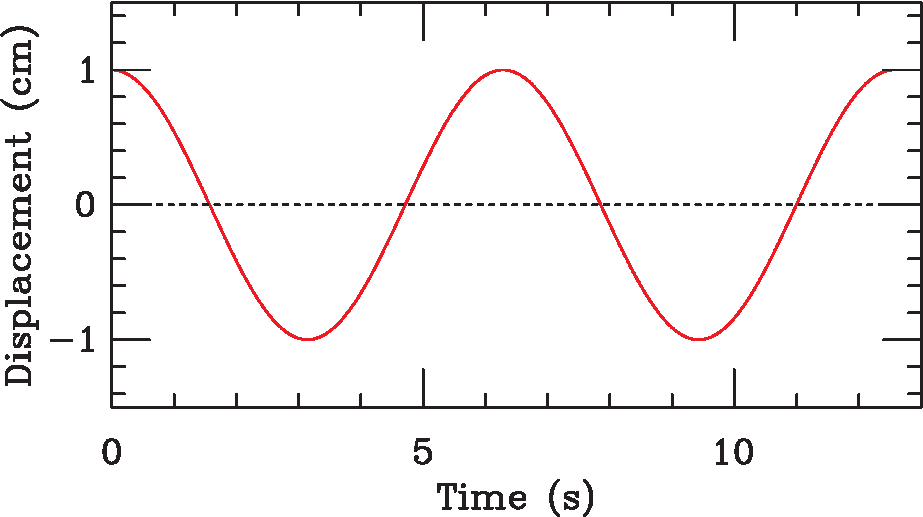
\includegraphics [width=\textwidth]{plot11.pdf}
\end{minipage}

\newpage

Note that since one complete cycle is $2\pi$ radians, the period $\tau$ of an oscillation is given by $\tau = \frac{2\pi}{\omega}$.

Suppose that you have a mass of $m = 10$ kg attached to a spring with a spring constant of $k = 40$ N/m. Someone pulls the mass a distance 5 cm to the side and releases it. Determine the following:

\bigskip

\begin{minipage}{0.25\textwidth}
	Amplitude $A$
\end{minipage}
\begin{minipage}{0.25\textwidth}
	Angular frequency $\omega$
\end{minipage}
\begin{minipage}{0.35\textwidth}
	Description of motion $x(t)$
\end{minipage}
\begin{minipage}{0.25\textwidth}
	Period $\tau$
\end{minipage}

\vspace{1.5in}

\begin{minipage}{0.5\textwidth}
On the axes below, sketch a graph of its position vs. time.
\bigskip

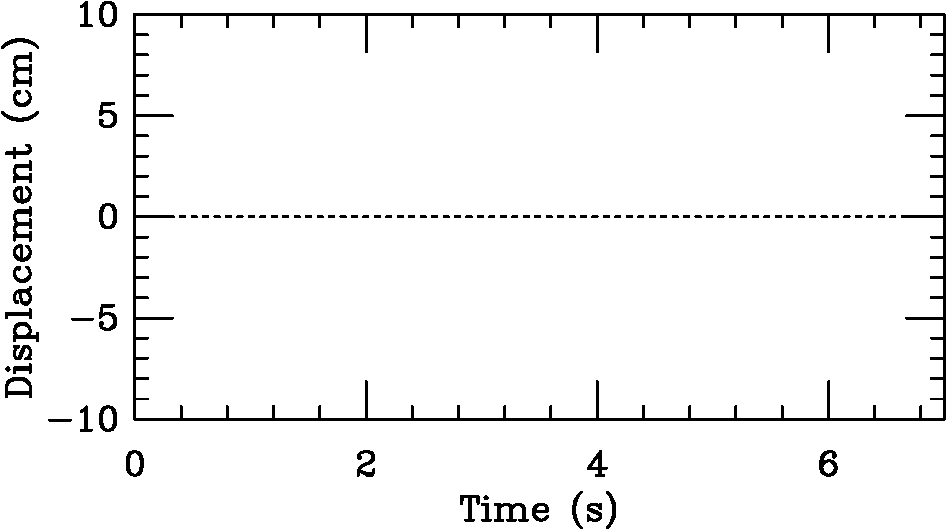
\includegraphics[width=0.7\textwidth]{blank.pdf}
\end{minipage}
\begin{minipage}{0.5\textwidth}
In this situation, you chose to use either sine or cosine for the equation describing the motion. Why did you make the choice that you did? Can you think of a physical scenario where you would use the other function instead? {\it (In other words, instead of pulling the mass to the side and releasing it, what would you have to do to it?)}
\vspace{2in}

\end{minipage}






 \end{document}
